% Preamble
%
% Installed this: http://ctan.math.washington.edu/tex-archive/systems/windows/protext/
% Useful shit:
% https://www.overleaf.com/4748747hgqdpz#/14481747/
% http://users.dickinson.edu/~richesod/latex/latexcheatsheet.pdf
%
% Useful graphics shit:
% http://tex.stackexchange.com/questions/16207/image-from-includegraphics-showing-up-in-wrong-location
% ---
\documentclass{article} % this is responsible for title on same page as rest
%\documentclass{report}
% Packages

% ---
% DO NOT use \usepackage{} in main document
\usepackage{amsmath} % Advanced math typesetting
%\usepackage[utf8]{inputenc} % Unicode support (Umlauts etc.)
%\usepackage[ngerman]{babel} % Change hyphenation rules
%\usepackage{hyperref} % Add a link to your document
\usepackage{graphicx} % Add pictures to your document
%\usepackage{listings} % Source code formatting and highlighting
\usepackage[framed,numbered,autolinebreaks,useliterate]{mcode}
\usepackage{Python}
\usepackage{graphicx}
\graphicspath{ {img/} }

\usepackage{hyperref}

% Main Document
\begin{document}
	\author{Michael Saybolt}
	\title{ECE 802 - 603: Microwave and Milimeter Waves: Homework 1}
	\date{3/29/2016} % Use \today{}
	\maketitle
	
	%\\ % Line break
	Learning how to use \LaTeX{}!
	
	\newpage{} % Page break
	
	\tableofcontents{} % Gen table of contents from sections
	
	\section{De-Embedding Data}
	De-embedding data will take measured S-parameters of a system and give us the S-parameters of the DUT without the error induced by the connection to the device.  Once measured data is acquired for the DUT, and control measurements for an open connection (no DUT), a short (to ground), and through (a section of line), the S-parameters of the error, or error boxes can be calculated.  From there, the inverse of the error box is multiplied by the S-parameters of the DUT, and then by the non-inverted S-parameters of the error box, assuming that the error boxes are symmetric.  The result is the de-embedded S-parameters of the DUT.  The following explains this procedure in greater detail.
	
	\subsection{Error Box S-parameters} \label{ssec:errorBox}
	The procedure for getting the S-parameters of the error box is found around/on p. 201 of Pozar's Microwave Engineering. Since $S_{11} = S_{22}$, and $S_{12} = S_{21}$, the equations are combined and $S_{11}$ and $S_{12}$ for the error box are obtained:
	
	\begin{align}
	S_{11_{Error}} = \frac{S_{11_{Short}} - 2*S_{11_{Through}} + S_{11_{Open}}}{S_{11_{Open}} - 2*S_{12_{Through}} - S_{11_{Short}}}
	\end{align}
	\begin{align}
	S_{12_{Error}} = \sqrt{S_{12_{Through}} * (1-S_{11_{Error}}^2)}
	\end{align}
	\begin{align}
	S_{21_{Error}} = S_{12_{Error}}
	\end{align}
	\begin{align}
	S_{22_{Error}} = S_{11_{Error}}
	\end{align}
	\subsection{De-embedding without MATLAB RF Toolbox} 
	The first time around, it was not known that MATLAB has an RF toolkit that does many of the things in this assignment.  Since 90\% of the time was spent doing it that way, the works are still presented. 
	\subsubsection{Functions}
	A MATLAB function was made to import .s2p files into an array type in MATLAB. It should be noted that the *.s2p import function had trouble with a s2p file so the files had to be modified in Notepad and the headers removed.  It appeared that the $importdata$ function in MATLAB only supports one type of comment line, and having lines that started with "\!" as well as "\#" resulted in confusion and data loss.
	
	\begin{lstlisting}[language=Matlab, caption=*.s2p Import]
	function [ S11, S21, S12, S22, freq ] = ECE802_S2Pread( fileName )
	%Read full S2P matrix
	%Note: make modified files with headers it knows how to deal with
	%      - More than one type of "comment" lines seems to confuse importdata
	
	[A, delimiterOut, headerlinesOut] = importdata(fileName);
	
	%import each column of data part of struct into vectors/matricies
	freq = A.data(:,1);
	
	S11(:,1) = A.data(:,2);
	S11(:,2) = A.data(:,3);
	
	S21(:,1) = A.data(:,4);
	S21(:,2) = A.data(:,5);
	
	S12(:,1) = A.data(:,6);
	S12(:,2) = A.data(:,7);
	
	S22(:,1) = A.data(:,8);
	S22(:,2) = A.data(:,9);
	end
	\end{lstlisting}
	
	More functions were made to convert S-parameters to ABCD parameters in order to perform the de-embedding operations on them, and then to convert ABCD back to S-parameters.
	
	\begin{lstlisting}[language=Matlab, caption=S-parameters to ABCD]
	function [ ABCD ] = StoABCD( S, Z0 )
	% StoABCD convert S matrix to ABCD parameters
	% V1.0
	% [A, B; C, D] = [S11, S12; S21, S22]
	
	ABCD(1,1) = ((1+S(1,1))*(1-S(2,2))+S(1,2)*S(2,1))/(2*S(2,1));
	ABCD(1,2) = Z0*((1+S(1,1)*(1+S(2,2))-S(1,2)*S(2,1))/(2*S(2,1)));
	ABCD(2,1) = 1/Z0*(((1-S(1,1))*(1-S(2,2))-S(1,2)*S(2,1))/(2*S(2,1)));
	ABCD(2,2) = (((1-S(1,1))*(1+S(2,2))+S(1,2)*S(2,1))/(2*S(2,1)));
	
	end
	\end{lstlisting}
	
	\begin{lstlisting}[language=Matlab, caption=ABCD to S-parameters]
	function [ S ] = ABCDtoS( ABCD, Z0 )
	% ABCDtoS convert ABCD mat to Spara
	% V1.0
	% [S11, S12; S21, S22] = [A, B; C, D]
	
	% reassign for readability and ease of coding
	A = ABCD(1,1); B = ABCD(1,2); C = ABCD(2,1); D = ABCD(2,2);
	
	S(1,1) = (A + B/Z0 - C*Z0 - D)/(A + B/Z0 + C*Z0 + D);
	S(1,2) = (2*(A*D - B*C))/(A + B/Z0 + C*Z0 + D);
	S(2,1) = 2/(A + B/Z0 + C*Z0 + D);
	S(2,2) = (-A + B/Z0 - C*Z0 + D)/(A + B/Z0 + C*Z0 + D);
	
	end	
	\end{lstlisting}
	
	\subsubsection{Main Code}
	These functions are called repeatedly inside the main body of the code.  Most of it runs inside a giant $for$ loop that does the de-embedding operation on a 2x2 matrix for each frequency.  These are assembled at the end back into the 2x2xN matrix for plotting along the frequency slice. 
	
	\begin{lstlisting}[language=Matlab, caption=De-embedding MATLAB Code]
	%802 deembedding shit draft
	%folderName = [pwd,'\De-Embedding Data']
	
	clear; close all;
	
	% LDR Data
	[DiodeS11, DiodeS21, DiodeS12, DiodeS22, freq] = ECE802_S2Pread('diode_mod.s2p');
	[OpenS11, OpenS21, OpenS12, OpenS22] = ECE802_S2Pread('open_mod.s2p');
	[ResistorS11, ResistorS21, ResistorS12, ResistorS22] = ECE802_S2Pread('resistor_mod.s2p');
	[ShortS11, ShortS21, ShortS12, ShortS22] = ECE802_S2Pread('short_mod.s2p');
	[ThroughS11, ThroughS21, ThroughS12, ThroughS22] = ECE802_S2Pread('through_mod.s2p');
	
	Z0 = 50;
	
	%Whole program is contained in for loop and runs for each frequency
	for ii = 1:length(freq)
	%Convert used data from mag<phase to re+j*im
	%DiodeS(ii,1,1) = magphase2cplex(DiodeS11(ii,1), DiodeS11(ii,2))
	DiodeS(ii,1,1) = db2magPwr(DiodeS11(ii,1))*exp(db2magPwr(DiodeS11(ii,2))*sqrt(-1));
	DiodeS(ii,2,1) = db2magPwr(DiodeS21(ii,1))*exp(db2magPwr(DiodeS21(ii,2))*sqrt(-1));
	DiodeS(ii,1,2) = db2magPwr(DiodeS12(ii,1))*exp(db2magPwr(DiodeS12(ii,2))*sqrt(-1));
	DiodeS(ii,2,2) = db2magPwr(DiodeS22(ii,1))*exp(db2magPwr(DiodeS22(ii,2))*sqrt(-1));
	
	ResistorS(ii,1,1) = db2magPwr(ResistorS11(ii,1))*exp(db2magPwr(ResistorS11(ii,2))*sqrt(-1));
	ResistorS(ii,2,1) = db2magPwr(ResistorS21(ii,1))*exp(db2magPwr(ResistorS21(ii,2))*sqrt(-1));
	ResistorS(ii,1,2) = db2magPwr(ResistorS12(ii,1))*exp(db2magPwr(ResistorS12(ii,2))*sqrt(-1));
	ResistorS(ii,2,2) = db2magPwr(ResistorS22(ii,1))*exp(db2magPwr(ResistorS22(ii,2))*sqrt(-1));
	
	ThroughS(ii,1,1) = db2magPwr(ThroughS11(ii,1))*exp(db2magPwr(ThroughS11(ii,2))*sqrt(-1));
	ThroughS(ii,2,1) = db2magPwr(ThroughS21(ii,1))*exp(db2magPwr(ThroughS21(ii,2))*sqrt(-1));
	ThroughS(ii,1,2) = db2magPwr(ThroughS12(ii,1))*exp(db2magPwr(ThroughS12(ii,2))*sqrt(-1));
	ThroughS(ii,2,2) = db2magPwr(ThroughS22(ii,1))*exp(db2magPwr(ThroughS22(ii,2))*sqrt(-1));
	
	OpenS(ii,1,1) = db2magPwr(OpenS11(ii,1))*exp(db2magPwr(OpenS11(ii,2))*sqrt(-1));
	OpenS(ii,2,1) = db2magPwr(OpenS11(ii,1))*exp(db2magPwr(OpenS11(ii,2))*sqrt(-1));
	OpenS(ii,1,2) = db2magPwr(OpenS11(ii,1))*exp(db2magPwr(OpenS11(ii,2))*sqrt(-1));
	OpenS(ii,2,2) = db2magPwr(OpenS11(ii,1))*exp(db2magPwr(OpenS11(ii,2))*sqrt(-1));
	
	ShortS(ii,1,1) = db2magPwr(ShortS11(ii,1))*exp(db2magPwr(ShortS11(ii,2))*sqrt(-1));
	ShortS(ii,2,1) = db2magPwr(ShortS11(ii,1))*exp(db2magPwr(ShortS11(ii,2))*sqrt(-1));
	ShortS(ii,1,2) = db2magPwr(ShortS11(ii,1))*exp(db2magPwr(ShortS11(ii,2))*sqrt(-1));
	ShortS(ii,2,2) = db2magPwr(ShortS11(ii,1))*exp(db2magPwr(ShortS11(ii,2))*sqrt(-1));
	
	Test(ii) = db2magPwr(ResistorS11(ii,1))*exp(db2magPwr(ResistorS11(ii,2))*sqrt(-1));
	%Test(ii,1,1) = db2magPwr(ResistorS11(ii,1))*exp(db2mag(ResistorS11(ii,2))*sqrt(-1));
	%Test(ii,2,1) = ResistorS21(ii,1)*exp(ResistorS21(ii,2)*sqrt(-1));
	
	% Solve:
	% Analytical Work: (P201 Pozar)
	% T11 = S11 + S22(S12^2/(1-S22^2)), S11 = S12
	% T12 = (S12^2/(1-S22^2))
	%
	% T11 = S11 + S22*T12 = S22(1+T12)  
	% ==>  S22 = T11/(1+T12)
	%
	% S12^2 = T12*(1-S22^2) = T12(1-(T11/(1+T12))^2)
	% ==> S12 = sqrt(T12(1-(T11/(1+T12))^2)) = sqrt(T12(1-S22^2))
	
	% Get Error box S param
	ErrorS(ii,1,1) = (ShortS(ii,1,1)-2*ThroughS(ii,1,1)+OpenS(ii,1,1))/ ...
	(OpenS(ii,1,1)-2*ThroughS(ii,1,2)-ShortS(ii,1,1));
	ErrorS(ii,1,2) = sqrt(ThroughS(ii,1,2)*(1-ErrorS(ii,1,1)^2));
	ErrorS(ii,2,1) = ErrorS(ii,1,2);
	ErrorS(ii,2,2) = ErrorS(ii,1,1);
	
	% Convert all shit to ABCD to manipulate
	%When drawing data from one 2x2 slice of n x m x p ubermatrix, use squeeze to
	%form the 2x2 (otherwise is a row of 4 elements for some stupid reason)
	%ResistorABCD(ii,:,:) = StoABCD(squeeze(ResistorS(ii,:,:)),Z0);
	ResistorABCD(ii,:,:) = s2a(squeeze(ResistorS(ii,:,:)));
	DiodeABCD(ii,:,:) = StoABCD(squeeze(DiodeS(ii,:,:)),Z0);
	ErrorABCD(ii,:,:) = StoABCD(squeeze(ErrorS(ii,:,:)),Z0);
	%%% ASK DR CHAHAL WHY USE INVERSE AGAIN (see p202 Pozar) %%%   
	ErrorDBCA(ii,:,:) = [ErrorABCD(ii,1,1) ErrorABCD(ii,1,2); ...
	ErrorABCD(ii,2,1) ErrorABCD(ii,2,2)];
	
	%De-embed
	%ResistorDemABCD(ii,:,:) = squeeze(ErrorABCD(ii,:,:))\ ...
	%squeeze(ResistorABCD(ii,:,:))/squeeze(ErrorABCD(ii,:,:));
	ResistorDemABCD(ii,:,:) = inv(squeeze(ErrorABCD(ii,:,:)))* ...
	squeeze(ResistorABCD(ii,:,:))*inv(squeeze(ErrorDBCA(ii,:,:)));
	
	
	%DiodeDemABCD(ii,:,:) = squeeze(ErrorABCD(ii,:,:))\ ...
	%squeeze(DiodeABCD(ii,:,:))/squeeze(ErrorABCD(ii,:,:));
	DiodeDemABCD(ii,:,:) = inv(squeeze(ErrorABCD(ii,:,:)))* ...
	squeeze(DiodeABCD(ii,:,:))*inv(squeeze(ErrorDBCA(ii,:,:)));
	
	% Convert back to S parameters
	%ResistorDemS(ii,:,:) = ABCDtoS(squeeze(ResistorDemABCD(ii,:,:)),Z0);
	ResistorDemS(ii,:,:) = a2s(squeeze(ResistorDemABCD(ii,:,:)));
	DiodeDemS(ii,:,:) = ABCDtoS(squeeze(DiodeDemABCD(ii,:,:)),Z0);
	end
	
	% Plot
	plottr(freq, ResistorS11(:,1),'Frequency (Hz)', '|S11|', 'Resistor S11(nonimbed, straight mag from file)')
	%plottr(freq, mag2dbPwr(sqrt(real(Test(:)).^2+imag(Test(:)).^2)), 'Frequency (Hz)', '|S11|', 'Resistor S11(test)')
	plottr(freq, mag2dbPwr(abs(Test(:))), 'Frequency (Hz)', '|S11|', 'Resistor S11(nonimbed, db->mag,mag->db)')
	
	%plottr(freq, abs(Test(:,2,1)), 'Frequency (Hz)', '|S21|', 'Resistor S21(test)')
	%Spara resistor
	plottr(freq, mag2dbPwr(abs(ResistorDemS(:,1,1))), 'Frequency (Hz)', '|S11|', 'Resistor S11')
	plottr(freq, mag2dbPwr(abs(ResistorDemS(:,1,2))), 'Frequency (Hz)', '|S12|', 'Resistor S12')
	plottr(freq, abs(ResistorDemS(:,2,1)), 'Frequency (Hz)', '|S21|', 'Resistor S21')
	plottr(freq, abs(ResistorDemS(:,2,2)), 'Frequency (Hz)', '|S22|', 'Resistor S22')
	
	%Spara diode
	plottr(freq, abs(DiodeDemS(:,1,1)), 'Frequency (Hz)', '|S11|', 'Diode S11')
	plottr(freq, abs(DiodeDemS(:,1,2)), 'Frequency (Hz)', '|S12|', 'Diode S12')
	plottr(freq, abs(DiodeDemS(:,2,1)), 'Frequency (Hz)', '|S21|', 'Diode S21')
	plottr(freq, abs(DiodeDemS(:,2,2)), 'Frequency (Hz)', '|S22|', 'Diode S22')
	
	% Export data for ADS
	filename = 'ResistorSpara.xlsx';
	xlswrite(filename,[freq,abs(ResistorDemS(:,1,1)),angle(ResistorDemS(:,1,1)), ...
	abs(ResistorDemS(:,1,2)), angle(ResistorDemS(:,1,2)), abs(ResistorDemS(:,2,1)), ...
	angle(ResistorDemS(:,2,1)), abs(ResistorDemS(:,2,2)), angle(ResistorDemS(:,2,2))]);
	
	filename = 'DiodeSpara.xlsx';
	xlswrite(filename,[freq,abs(DiodeDemS(:,1,1)),angle(DiodeDemS(:,1,1)), ...
	abs(DiodeDemS(:,1,2)), angle(DiodeDemS(:,1,2)), abs(DiodeDemS(:,2,1)), ...
	angle(DiodeDemS(:,2,1)), abs(DiodeDemS(:,2,2)), angle(DiodeDemS(:,2,2))]);
	\end{lstlisting}
	
	\subsubsection{Postprocessing with Excel and Python}
	The output of the MATLAB code is in .xls format for Microsoft Excel.  It needs to be converted back to .s2p for importing into ADS to make an equivalent model.
	
	First, the file is opened in Excel, and saved as a comma delimited file, *.csv.
	
	A Python script was made by Chris Oakley to convert *.csv to *.s1p for some other application called "csv\_to\_s1p.py".  It was modified a bit to accept more inputs and re-branded as "csv\_to\_s2p.py". This version of the script also accepts user input through the command prompt to specify the input and output filenames, however the working directory still must be specified in the file.  Below is the code.
	
	\begin{lstlisting}[language=Python, caption=Python Based *.csv to *.s2p Converter]
	# -*- coding: utf-8 -*-
	"""
	Created on Mon Feb 15 10:58:19 2016
	
	@author: oakleych
	@s2p_modder: sayboltm
	csv_to_s2p.py
	note: Crude but it works
	"""
	
	import os.path
	
	def getNumLines(fname, skiprows):
	lines = 0        
	
	if os.path.isfile(fname):
	f = open(fname, 'r')
	
	for n in range(skiprows):
	f.readline()
	
	for line in f:
	if line[0] == 'E':
	break
	else:
	lines += 1
	
	f.close()
	
	return lines
	
	num_ports = 1
	
	
	#Set this to the directory where the data is stored
	#basedir = r"M:\SiCRFPAPER\spara/"
	basedir = r"C:\Users\Mike\Dropbox\Documents\MS EE\SS16\ECE 802 - 603 (MWndMM Ciruits)\HW\HW1/"
	print('Present working directory is:\n', basedir)
	
	#Input file name
	#csv_name = 'ResistorSpara.csv'
	print('\nInput file to get converted including .csv extension:')
	csv_name = input()
	
	#Output file name
	#out_name = 'ResistorSpara.s2p'
	print('\nInput desired output file name, again with extension:')
	out_name = input()
	
	# Note the 8 at the end that skips some lines
	data_lines = getNumLines(basedir + csv_name, 8)
	
	csv_file = open(basedir + csv_name, 'r')
	
	#Number of comment lines in CSV file
	comment_rows = 5
	
	comment_lines = ''
	freq_data = []
	mag_data11 = []
	phase_data11 = []
	mag_data12 = []
	phase_data12 = []
	mag_data21 = []
	phase_data21 = []
	mag_data22 = []
	phase_data22 = []
	
	# Suck up the comments for use later
	for i in range(comment_rows):
	comment_lines += csv_file.readline()
	
	#discard empty line
	tmp = csv_file.readline()
	
	#discard BEGIN line    
	tmp = csv_file.readline()
	
	#Get header information
	hdr_line = csv_file.readline()
	hdr = hdr_line.split(',')
	
	#Get frequency units
	freq_unit = hdr[0].split('(')
	freq_unit = freq_unit[1].split(')')
	freq_unit = freq_unit[0]
	
	#Get channel name and type
	ch_info = hdr[1]
	ch_info = ch_info.split('(')
	ch_name = ch_info[0]
	ch_unit = ch_info[1].split(')')
	ch_unit = ch_unit[0]
	
	#Change case if not set properly
	if ch_unit == 'DB':
	ch_unit = 'dB'
	
	#Read in data from CSV file
	for i in range(data_lines):
	line = csv_file.readline()
	line = line.split(',')
	
	freq_data.append(line[0])
	mag_data11.append(line[1])
	phase_data11.append(line[2])
	mag_data12.append(line[3])
	phase_data12.append(line[4])
	mag_data21.append(line[5])
	phase_data21.append(line[6])
	mag_data22.append(line[7])
	phase_data22.append(line[8])
	
	
	csv_file.close()
	
	out_file = open(basedir + out_name, 'w+')
	
	#Output format line to write data
	format_line = '# ' + freq_unit + ' S ' + ch_unit + ' R 50' + '\n'
	
	#Include channel name
	snp_comment = '!S2P File: Measurements:(justKiddingNotChannelname) ' + ch_name + '\n'
	comment_lines += snp_comment
	#can put moar shit here if gather moar channel names
	
	#Write out comments and format information
	out_file.writelines(comment_lines) #restore the comments
	out_file.writelines(format_line) #print the format stuff with units/whatever
	
	#Write data
	for i in range(len(freq_data)):
	line_out = freq_data[i] + ' ' + mag_data11[i] + ' ' + phase_data11[i] + ' ' + mag_data12[i] + ' ' + phase_data12[i] + ' ' + mag_data21[i] + ' ' + phase_data21[i]+ ' ' + mag_data22[i] + ' ' + phase_data22[i]# + '\n'
	out_file.writelines(line_out)
	
	
	out_file.close()
	
	print('Operation completed successfully.')
	\end{lstlisting}
	
	The script outputs the *.s2p file ready to import into ADS!
	
	\subsection{De-embedding with MATLAB RF Toolbox}
	This was much easier, and the second (current) version was able to be done without a single $for$ loop!  Data is imported into "rfdata" objects through built-in functions designed for *.s2p files.  No manual editing is necessary.  Error box S-parameters are obtained as described in \autoref{ssec:errorBox}.
	
	S-parameters are extracted, and the error box and DUT S-parameters are fed into a de-embed function, part of the RF Toolbox.  Conversion from S-parameters to ABCD is done inside the function, however the dB conversion only goes one way, so $20*log10(x)$ must be applied to convert back to dB before plotting.  This entire process was much more simple.  Below is the code.
	
	\begin{lstlisting}[language=Matlab, caption=De-embedding with RF Toolbox]
	%ECE802Deembedder3
	% IT works and is simple!
	
	clear; close all;
	
	Diode = read(rfdata.data, 'diode.s2p');
	Resistor = read(rfdata.data, 'resistor.s2p');
	Open = read(rfdata.data, 'open.s2p');
	Short = read(rfdata.data, 'short.s2p');
	Through = read(rfdata.data, 'through.s2p');
	
	%DiodeS = sparameters(Diode);
	[DiodeS, freq]  = extract(Diode, 'S_parameters');
	ResistorS = extract(Resistor, 'S_parameters');
	OpenS = extract(Open, 's_parameters');
	ShortS = extract(Short, 's_parameters');
	ThroughS = extract(Through, 's_parameters');

	% Get Error box S param
	ErrorS(1,1,:) = (ShortS(1,1,:)-2.*ThroughS(1,1,:)+OpenS(1,1,:))./ ...
	(OpenS(1,1,:)-2.*ThroughS(1,2,:)-ShortS(1,1,:));
	ErrorS(1,2,:) = sqrt(ThroughS(1,2,:).*(1-ErrorS(1,1,:).^2));
	ErrorS(2,1,:) = ErrorS(1,2,:);
	ErrorS(2,2,:) = ErrorS(1,1,:);
	
	ResistorDemS = deembedsparams(ResistorS, ErrorS, ErrorS);
	DiodeDemS = deembedsparams(DiodeS, ErrorS, ErrorS);
	
	% Plot stuff
	% Note that, for some reason matlab is not psychic and assumes your data
	% are not power measurements so it does 20log10 instead of 10log10.  Or
	% maybe Saran wrap was wrong and it should be 20log10. Dunno.
	plottr(freq, mag2db(squeeze(abs(ResistorS(1,1,:)))), 'Frequency (Hz)', '|S11|', 'Resistor S11')
	hold on
	plot(freq, mag2db(squeeze(abs(ResistorDemS(1,1,:)))),  'g')
	legend('Original', 'Deembedded')
	
	plottr(freq, mag2db(squeeze(abs(ResistorS(1,2,:)))), 'Frequency (Hz)', '|S12|', 'Resistor S12')
	hold on
	plot(freq, mag2db(squeeze(abs(ResistorDemS(1,2,:)))),  'g')
	legend('Original', 'Deembedded')
	
	plottr(freq, mag2db(squeeze(abs(ResistorS(2,1,:)))), 'Frequency (Hz)', '|S21|', 'Resistor S21')
	hold on
	plot(freq, mag2db(squeeze(abs(ResistorDemS(2,1,:)))),  'g')
	legend('Original', 'Deembedded')
	
	plottr(freq, mag2db(squeeze(abs(ResistorS(2,2,:)))), 'Frequency (Hz)', '|S22|', 'Resistor S22')
	hold on
	plot(freq, mag2db(squeeze(abs(ResistorDemS(2,2,:)))),  'g')
	legend('Original', 'Deembedded')
	
	
	plottr(freq, mag2db(squeeze(abs(DiodeS(1,1,:)))), 'Frequency (Hz)', '|S11|', 'Diode S11')
	hold on
	plot(freq, mag2db(squeeze(abs(DiodeDemS(1,1,:)))),  'g')
	legend('Original', 'Deembedded')
	
	plottr(freq, mag2db(squeeze(abs(DiodeS(1,2,:)))), 'Frequency (Hz)', '|S12|', 'Diode S12')
	hold on
	plot(freq, mag2db(squeeze(abs(DiodeDemS(1,2,:)))),  'g')
	legend('Original', 'Deembedded')
	
	plottr(freq, mag2db(squeeze(abs(DiodeS(2,1,:)))), 'Frequency (Hz)', '|S21|', 'Diode S21')
	hold on
	plot(freq, mag2db(squeeze(abs(DiodeDemS(2,1,:)))),  'g')
	legend('Original', 'Deembedded')
	
	plottr(freq, mag2db(squeeze(abs(DiodeS(2,2,:)))), 'Frequency (Hz)', '|S22|', 'Diode S22')
	hold on
	plot(freq, mag2db(squeeze(abs(DiodeDemS(2,2,:)))),  'g')
	legend('Original', 'Deembedded')
	
	%write(ResistorDemS, 'demres.s2p')
	
	% Export to Excel, save as .csv, then use Python to convert to .s2p
	filename = 'ResistorSpara.xlsx';
	xlswrite(filename,[freq,mag2db(squeeze(abs(ResistorDemS(1,1,:)))), squeeze(angle(ResistorDemS(1,1,:))), ...
	mag2db(squeeze(abs(ResistorDemS(1,2,:)))), squeeze(angle(ResistorDemS(1,2,:))), mag2db(squeeze(abs(ResistorDemS(2,1,:)))), ...
	squeeze(angle(ResistorDemS(2,1,:))), mag2db(squeeze(abs(ResistorDemS(2,2,:)))), squeeze(angle(ResistorDemS(2,2,:)))]);
	
	filename = 'DiodeSpara.xlsx';
	xlswrite(filename,[freq,mag2db(squeeze(abs(DiodeDemS(1,1,:)))), squeeze(angle(DiodeDemS(1,1,:))), ...
	mag2db(squeeze(abs(DiodeDemS(1,2,:)))), squeeze(angle(DiodeDemS(1,2,:))), mag2db(squeeze(abs(DiodeDemS(2,1,:)))), ...
	squeeze(angle(DiodeDemS(2,1,:))), mag2db(squeeze(abs(DiodeDemS(2,2,:)))), squeeze(angle(DiodeDemS(2,2,:)))]);
	\end{lstlisting}
	
	\newpage{}
	
	\section{Agilent ADS Model}
	The exported *.s2p parameters were imported into Agilent ADS.
	
	\subsection{De-embedding Results}
	\subsubsection{Resistor}
	Figures 1 through 4 show the results of the de-embedding for the resistor, visualized in ADS:

	\begin{figure}[!ht] %h = try to keap near, t = top, b = bottom? ! = really try, H = don't move
	\begin{center}
		\label{fig:RS11}
	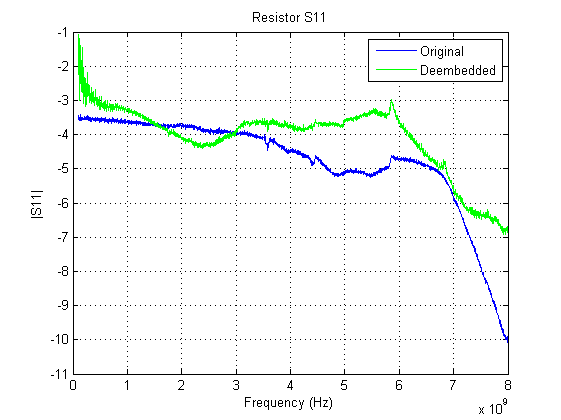
\includegraphics{ResistorS11}
	\caption{$Resistor S_{11}$}
	\end{center}
	\end{figure}
	
	\begin{figure}[H]
	\centering
	\label{fig:RS12}
	\caption{$Resistor S_{12}$}
	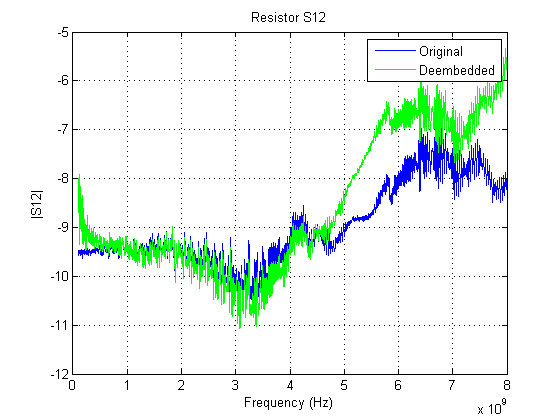
\includegraphics{ResistorS12}
	\end{figure}
	
	
	\begin{figure}[H]
		\centering
		\label{fig:RS21}
		\caption{$Resistor S_{21}$}
		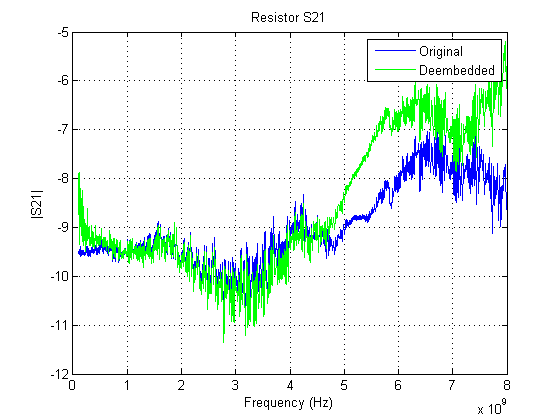
\includegraphics{ResistorS21}
	\end{figure}
	
	
	\begin{figure}[H]
		\centering
		\label{fig:RS22}
		\caption{$Resistor S_{22}$}
		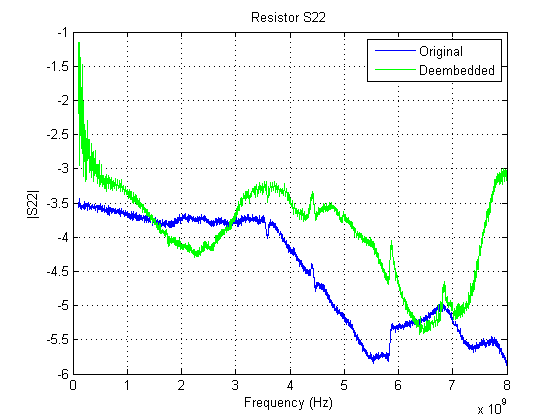
\includegraphics{ResistorS22}
	\end{figure}
	
	\vfill
	\clearpage
	
	\subsubsection{Diode} % WHy no worke? \autoref{fig:DS11} through \autoref{fig:DS22}
	Figures 5 through 8 show the results of the de-embedding for the diode.
	
	\begin{figure}[!h]
		\centering
		\label{fig:DS11}
		\caption{$Diode S_{11}$}
		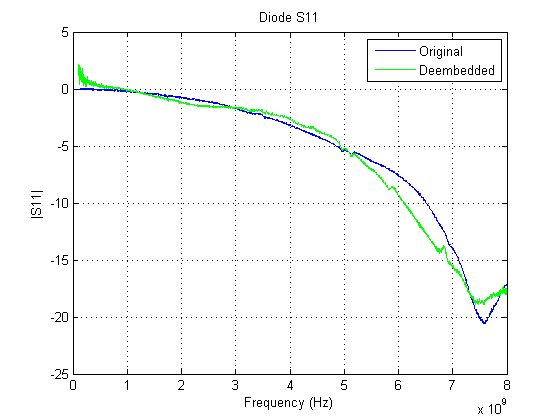
\includegraphics{DiodeS11}
	\end{figure}
	
	\begin{figure}[!H]
		\centering
		\label{fig:DS12}
		\caption{$Diode S_{12}$}
		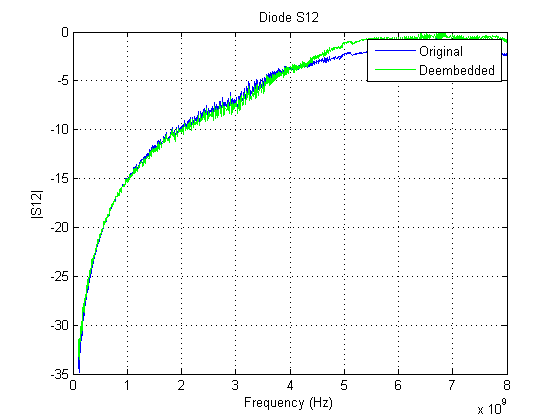
\includegraphics{DiodeS12}
	\end{figure}
	
	\begin{figure}[!H]
		\centering
		\label{fig:DS21}
		\caption{$Diode S_{21}$}
		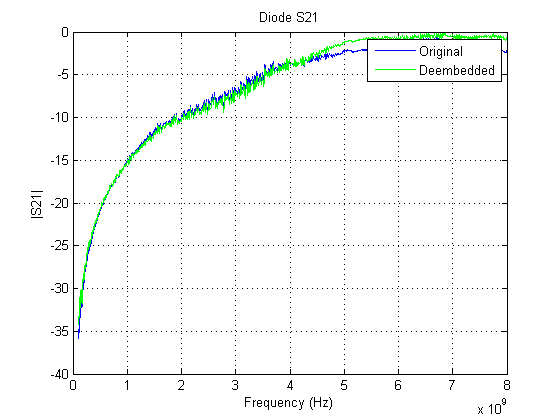
\includegraphics{DiodeS21}
	\end{figure}
	
	\begin{figure}[!H]
		\centering
		\label{fig:DS22}
		\caption{$Diode S_{22}$}
		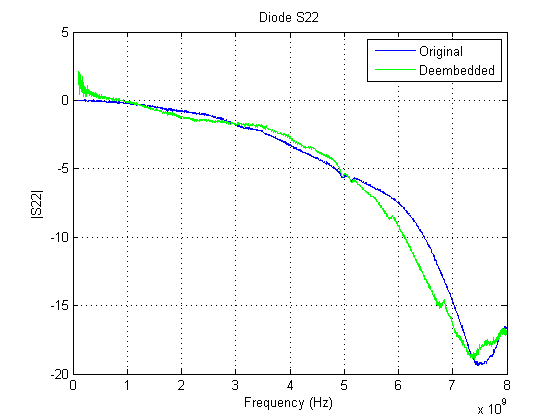
\includegraphics{DiodeS22}
	\end{figure}
	
	\vfill %vertically center the content
	\clearpage %no moar floats can cross this so graphs SHOULD be in the right spot (itworked!)
	
	\subsubsection{Observations}
	It is interesting to note that both the original and de-embedded signals for the resistor were much more noisy than that of the diode.  The ESR of the resistor is probably higher, since its resistor lumped element value was set to 203.75 $\Omega$ instead of 50 $\Omega$ like for the diode.  More resistance equates to more noise, but I would not expect that slight change to be visible here.  Then again, most of my experience dealing with noise such as this has been at audio frequencies in ECE 402.
	
	\subsection{Schematics and Models}
	After a basic equivalent model of the board and DUT were realized in ADS using t-lines and lumped elements, the tuning option was used to adjust the component values and see the resulting change in S-parameters of the system.
	
	\subsubsection{Resistor}
	Below is the best matching obtained for the resistor and its corresponding schematic with component values:
	
	\begin{figure}[h]
		\centering
		\caption{Resistor Matched to Measured Values}
		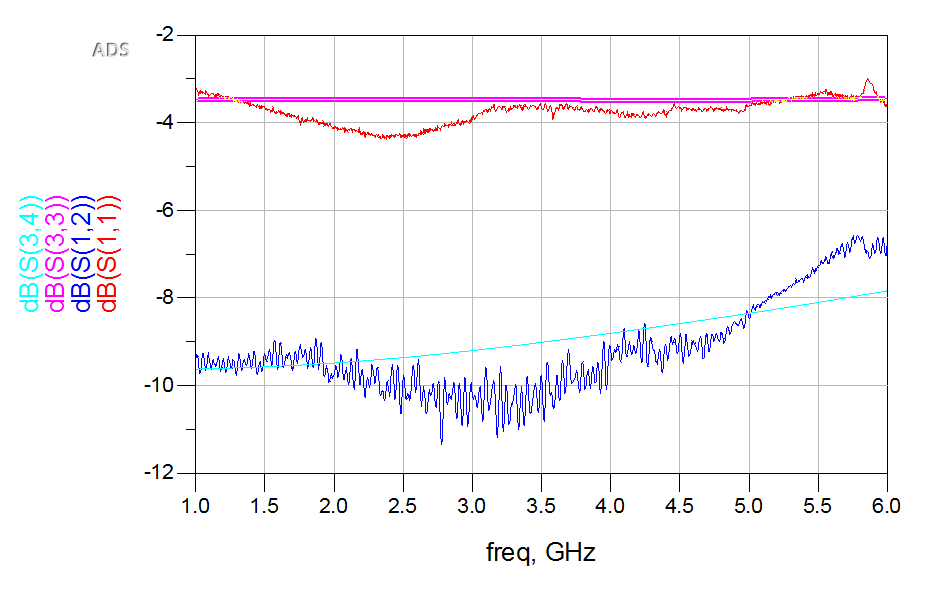
\includegraphics[scale=.6]{ResistorMatched}
	\end{figure}
	
	
	\begin{figure}[h]
		\centering
		\caption{Resistor Schematic with Updated Component Values}
		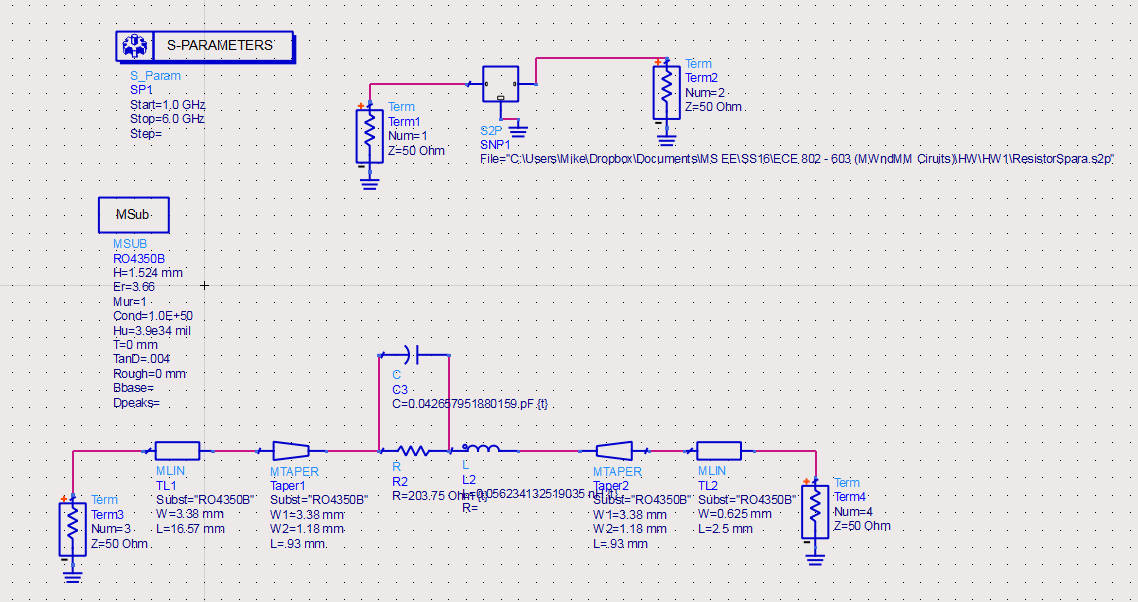
\includegraphics[scale=.5]{ResistorMatched_schematic}
	\end{figure}
	
	The resulting values are: \\
	R = 203.75 $\Omega$ \\
	C = 0.04266 pF \\
	L = 0.056234 nH
	
	\vfill
	\clearpage
	
	\subsubsection{Diode}
	Below are the results for the tuned diode model followed by the resulting component values:
	
	\begin{figure}[h]
		\centering
		\caption{Diode Matched to Measured Values}
		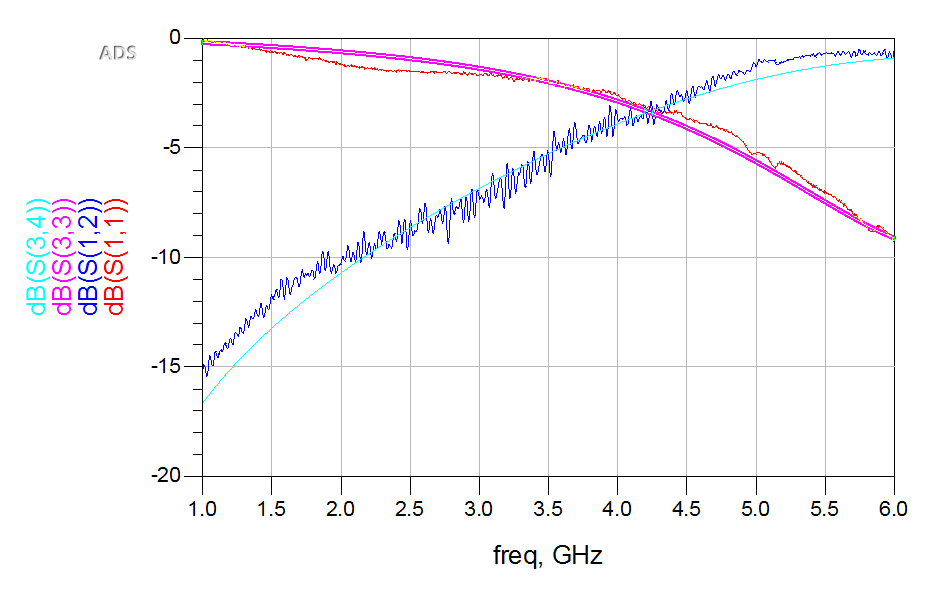
\includegraphics[scale=.6]{DiodeMatched}
	\end{figure}
	
	
	\begin{figure}[h]
		\centering
		\caption{Diode Schematic with Updated Component Values}
		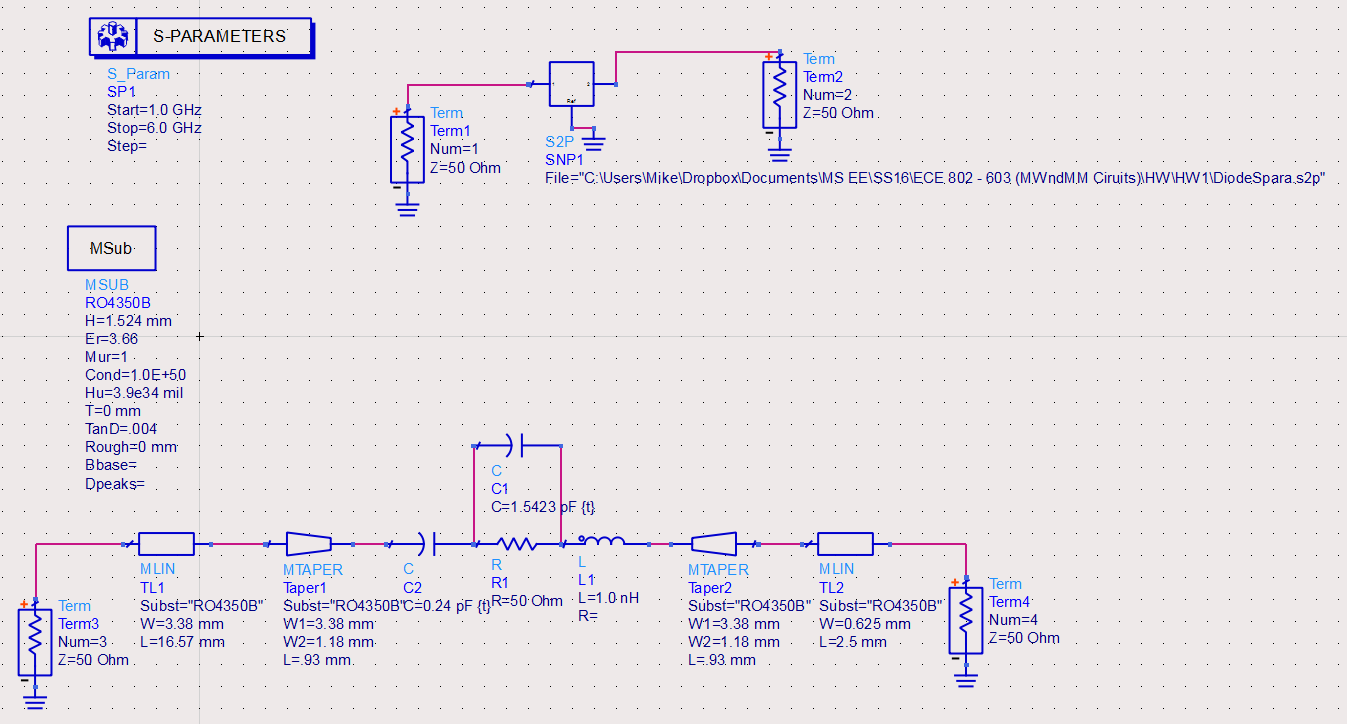
\includegraphics[scale=.45]{DiodeMatched_schematic}
	\end{figure}
	
	The resulting values are:\\
	R = 50 $\Omega$ \\
	C1 = 1.5423 pF (shunt C) \\
	C2 = 0.24 pF \\
	L = 1.0 nH
	
	\vfill
\end{document}